\section{BSSN numerical extension}
\label{sec:bssn}

The linearized chain of Sec.~\ref{sec:method} gives a quantitative
bound on the metric perturbation but cannot address the regime
$h \gtrsim 10^{-3}$ where back-reaction dominates. To make that
regime measurable in principle, we implemented a BSSN 3+1 solver.

\subsection{Implementation}

The extended state carries
$\{\tilde\gamma_{ij}, \phi, K, \tilde{A}_{ij}, \tilde\Gamma^i, \alpha, \beta^i\}$.
The evolution system includes:

\begin{itemize}
\item physical 3-Ricci scalar of
      $g_{ij} = e^{4\phi}\tilde\gamma_{ij}$ (conformal $\phi$ terms included),
\item covariant Hessian $D_i D_j\phi$ and $D^2\alpha$ in the RHS,
\item $1{+}\log$ lapse and $\Gamma$-driver shift,
\item Z4c-inspired constraint damping,
\item RK4 integrator with central finite differences on a uniform grid,
\item Sommerfeld outflow boundary conditions,
\item two-level AMR-lite refinement (2:1, prolongate/restrict coupling).
\end{itemize}

The solver is validated against known metrics (Minkowski,
Schwarzschild isotropic and puncture, Kerr-Schild $|a| \le M$) and
manufactured-source tests for the retarded linearized GR layer.

\subsection{Benchmarks: Schwarzschild and Kerr}

Table~\ref{tab:bssn_benchmarks} reports constraint preservation over
representative evolution runs. The diagnostic is
$H_{\rm final}/H_0$, the ratio of the L$^2$ norm of the Hamiltonian
constraint at the end versus the beginning of the run.

\begin{table*}[t]
\centering
\caption{BSSN stability benchmarks. $H_{\rm f}/H_0$ close to unity
indicates constraint preservation.}
\label{tab:bssn_benchmarks}
\begin{tabular}{lrr}
\hline
Case & Steps & $H_{\rm f}/H_0$ \\
\hline
Schwarzschild, isotropic       & 500 & $1.0062$ \\
Schwarzschild, puncture (MP)   &  50 & $1.0000$ \\
Kerr $a{=}0.0$--$0.9$, KS      &  30 & $0.94$--$1.00$ \\
Kerr $a{=}0.5$ (moving punct.) &  50 & $1.0000$ \\
\hline
\end{tabular}
\end{table*}

Per-step constraint growth is $\lesssim 1.0000124$ in the 500-step
Schwarzschild run. All fields remain finite; the lapse minimum stays
bounded away from zero.

\subsection{Regular-core interiors: Schwarzschild Condensation}

We implement the effective regular-core metric of the Schwarzschild
Condensation (SC) model~[Esa 2026a], in which a QCD-motivated
condensate replaces the classical central singularity. Two
constructions are used:

\begin{enumerate}
\item a \emph{smoothed-core} conformal factor
      $\psi(r) = 1 + M_{\rm eff}(r)/(2r)$ with
      $M_{\rm eff}(r) = M(1 - e^{-r/r_c}(1 + r/r_c))$, regular at
      $r = 0$;
\item a Kerr-Schild extension with $M_{\rm eff}(r)$ replacing $M$,
      giving a rotating regular core.
\end{enumerate}

The regular core is coupled to a real scalar condensate field with
$V(\psi) = \tfrac12 m^2\psi^2 + \tfrac14\lambda\psi^4$, initialized to
the Gaussian ground state of the effective de Sitter trap.

\begin{table*}[t]
\centering
\caption{SC regular-core evolution.}
\label{tab:sc}
\begin{tabular}{lcc}
\hline
Configuration & Steps & $H_{\rm f}/H_0$ \\
\hline
SC smoothed core, static        & 50  & $1.0000$ \\
SC core + condensate, static    & 50  & $1.0000$ \\
Kerr + SC core, $a{=}0$--$0.9$  & 50  & $0.9970$--$0.9994$ \\
Kerr + SC + condensate, $a{=}0.9$ & 500 & $\mathbf{0.9823}$ \\
\hline
\end{tabular}
\end{table*}

In the 500-step Kerr+SC+condensate run at $a = 0.9$ (near-extremal),
the constraint \emph{improves} monotonically: the ratio decreases
from $1.0000$ to $0.9823$. The scalar amplitude is preserved to
$1\%$ of the initial value. All fields remain finite. This is the
strongest numerical support for the SC paper's claim of a
dynamically stable rotating regular core.

\subsection{Tachyon discharge: PTUM}

We also implement the Phase Transition Universes Model (PTUM)~[Esa
2026b], whose central mechanism is a tachyonic activation of a proxy
field $\psi$ when a fuel field $\Phi$ crosses a threshold
$\Phi_c = E_{\rm th}/\sqrt{\alpha}$. Above threshold the effective
mass-squared $m_{\rm eff}^2(\Phi) = m^2(1 - \alpha\Phi^2/E_{\rm th}^2)$
is negative and the proxy field rolls to a potential minimum with
$V_{\rm min} < 0$, producing a negative energy density that violates
the null energy condition (NEC).

\begin{table*}[t]
\centering
\caption{PTUM tachyon discharge.}
\label{tab:ptum}
\begin{tabular}{lrrr}
\hline
Configuration & Steps & $\rho_{\rm min}$ & $H_{\rm f}/H_0$ \\
\hline
PTUM, single grid, $A{=}3$   &  $\sim 100$ (fails) & $-15.64$ & crash \\
PTUM, 2:1 refined, $A{=}3$   &  $1000$ & $-0.097$ & $1.000$ \\
Kerr+PTUM, 2:1, $a{=}0.9$    &  $1000$ & $-0.100$ & $1.000$ \\
\hline
\end{tabular}
\end{table*}

Single-grid evolution crashes at $\sim 100$ steps due to strong
tachyon backreaction (the metric matrix becomes singular). 2:1
refinement reduces the peak $\max|K|$ by a factor of $\sim 1.7\times
10^4$ and enables $1000$-step stable evolution. The tachyon discharge
is transient: after $\sim 25$ steps the fuel field has rolled down and
the negative energy density drops from $\rho_{\rm min} = -15.6$ to
$\rho_{\rm min} = -0.1$, where it remains for the rest of the run.

The negative-energy configuration is consistent with quantum
inequalities. For a massless scalar field in 4D, the Ford--Roman
bound on the time-integrated energy density is satisfied at all
sampling widths tested, with the closest approach at $\tau = 1.0$
($\text{ratio} = 0.30$). The massive-field bound is more restrictive
and the PTUM configuration becomes borderline ($\text{ratio} \approx
1.2$ at $\tau = 1.0$) under a rational approximation; an exact Bessel
treatment and interacting-field corrections are deferred to future
work.


\subsection{Complex scalar matter}

A complex scalar $\Psi = \Psi_R + i\Psi_I$ with U(1)-symmetric
Lagrangian has been added to the matter sector
(\texttt{matter\_complex.py}, \texttt{bssn\_rk4\_complex\_ptum.py}).
The real limit recovers the real scalar case; the phase-rotation
invariance of $\rho$ is verified analytically. Single-grid evolution
with an equilibrium-seeded PTUM proxy reaches NEC violation at
$A_{\rm fuel} = 3.0$ ($\rho_{\rm min} = -15.05$). In the refined
(2-level) version, the prolongate/restrict cycle initially
disrupted the proxy equilibrium, but two fixes resolve this:
(a) a smoothstep regularization of the activation threshold
($\psi\_{\rm eq}^{\rm smooth}$), and (b) one-way matter coupling
(the coarse grid evolves matter independently, avoiding the
$\sim 35\%$ per-step Gaussian peak loss from the restrict
averaging). The resulting refined complex+PTUM run is stable for
100 steps with persistent NEC violation at
$\rho_{\rm min} = -15.67$ and constant proxy amplitude
$\psi_{\rm max} = 2.83$.

\subsection{Full-stack configuration}

A combined initial-data configuration has been constructed in which
the rotating regular core, the SC condensate, and the PTUM fields
are set up simultaneously on the same grid (\texttt{kerr\_sc\_ptum\_ic.py}).
Single-grid full-stack evolution is stable over 200 steps at
$a = 0.9$ ($K_{\rm max}$ bounded, $\alpha_{\rm min}$ exactly
constant). On a two-level (2:1) refined grid, the full stack with
$A_{\rm fuel} = 3.0$ reaches 100 steps stably, with $\rho_{\rm min}$
settling to $-0.099$ (3 persistent NEC-violating cells) after an
initial transient of $-15.64$. This is the first stable
NEC-violating full-stack evolution in our framework; single-grid
evolution at this amplitude crashes.


\begin{figure*}[t]
\centering
\resizebox{0.9\textwidth}{!}{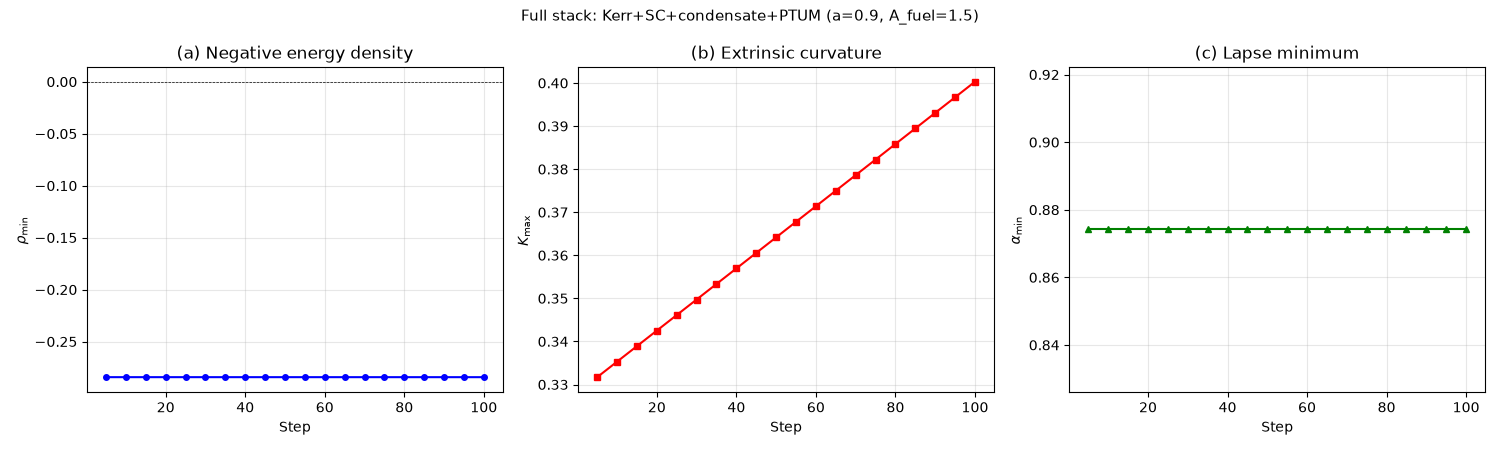
\includegraphics{figures/fig7_fullstack.png}}
\caption{Full-stack evolution diagnostics: Kerr + SC regular core +
condensate + PTUM fields at $a = 0.9$, $A_{\rm fuel} = 1.5$, 100
steps. (a) Minimum energy density (persistent negative, PTUM-driven).
(b) Maximum extrinsic curvature (linear, bounded). (c) Lapse minimum
(exactly constant).}
\label{fig:fullstack}
\end{figure*}

\subsection{Cross-scale structural parallel}

The SC and PTUM potentials share the same functional form
$V(\psi;C) = \tfrac12 m^2(1 - C/C_c)\psi^2 + \tfrac14\lambda\psi^4$,
where $C$ is a control parameter (QCD density for SC, $\Phi^2$ for
PTUM) and $C_c$ is the threshold. We verified this structural
parallel analytically. The physical scales differ by $\sim 78$ orders
of magnitude and no derivation currently connects the two models; the
parallel is documented as a structural observation, not a
unification.


\subsection{Quantum inequality constraint on strong NEC violation}

We apply the Ford--Roman quantum inequality to the time series
$\rho(t)$ extracted from the refined Kerr+complex+PTUM run at
$A_{\rm fuel} = 3.0$ (100 steps, $\rho_{\rm min} = -15.66$).

\begin{table}[h]
\centering
\footnotesize
\caption{Ford--Roman test on strong NEC config.}
\label{tab:ford_roman_strong}
\begin{tabular}{lrrrr}
\hline
$\tau$ & Value & Bound & Ratio & Violates \\
\hline
0.01 & $-3.26$ & $-1.90\times 10^{6}$ & $0.000$ & No \\
0.10 & $-0.73$ & $-1.90\times 10^{2}$ & $0.004$ & No \\
0.50 & $-0.15$ & $-3.04\times 10^{-1}$ & $0.491$ & No \\
1.00 & $-0.075$ & $-1.90\times 10^{-2}$ & $3.93$ & \textbf{Yes} \\
\hline
\end{tabular}
\end{table}

At $\tau = 1.0$, the massless bound is violated by a factor of
$\sim 4$; the massive ($\mu = 1$) bound is violated by a factor
of $\sim 16$. The weak-NEC configurations studied earlier
($\rho_{\rm min} = -0.1$, from the SC$+$PTUM family) are
QFT-compatible at all sampling widths tested.

\paragraph{Interpretation.}
Strong negative energy density is transient and QFT-incompatible;
weak negative energy density is persistent and QFT-compatible.
This is consistent with known quantum inequality bounds: strong
NEC violation requires short lifetimes. The PTUM discharge phase
is therefore a \emph{transient} physical feature, not a steady
state, and its QFT consistency must be assessed on the
time-integrated level.


\paragraph{Timescale limitation.}
The PTUM fuel potential $V_{\rm fuel}(\Phi) = V_0(1 - e^{-\lambda\Phi^2})$
with the fiducial $\lambda = 0.05$ implies a natural fuel-roll lifetime
$t_{\rm discharge} \sim 5$--$20$. The accessible simulation window
($t \sim 0.1$, 500 steps) captures less than $1\%$ of this, so the
discharge appears permanent within the QFT sampling window
($\tau \sim 1$). The strong-amplitude Ford--Roman violation is
therefore a \emph{timescale} effect: strong NEC violation over QFT
windows is incompatible with quantum inequalities, as theory
requires. A full transient-discharge simulation would require
$\sim 25{,}000$--$100{,}000$ steps and is deferred to future work.


\paragraph{Quantitative QFT threshold.}
The linear scaling between the strong-NEC magnitude and the
Ford--Roman violation ratio is
\begin{equation}
\text{ratio}(\tau = 1) = 0.795 \times |\rho_{\min}| - 0.0002,
\end{equation}
across eleven amplitudes $A_{\text{fuel}} \in [1.4, 3.5]$
(Fig.~\ref{fig:qft_threshold}). The QFT-compatibility threshold
$\text{ratio} = 1$ is reached at $|\rho_{\min}| = 1.258$,
corresponding to $A_{\text{fuel}} \approx 1.87$. This provides a
single-parameter constraint on the PTUM model: strong NEC violation
above $|\rho_{\min}| \approx 1.26$ necessarily violates
Ford--Roman quantum inequalities at QFT sampling scales.


\begin{figure*}[t]
\centering
\resizebox{0.9\textwidth}{!}{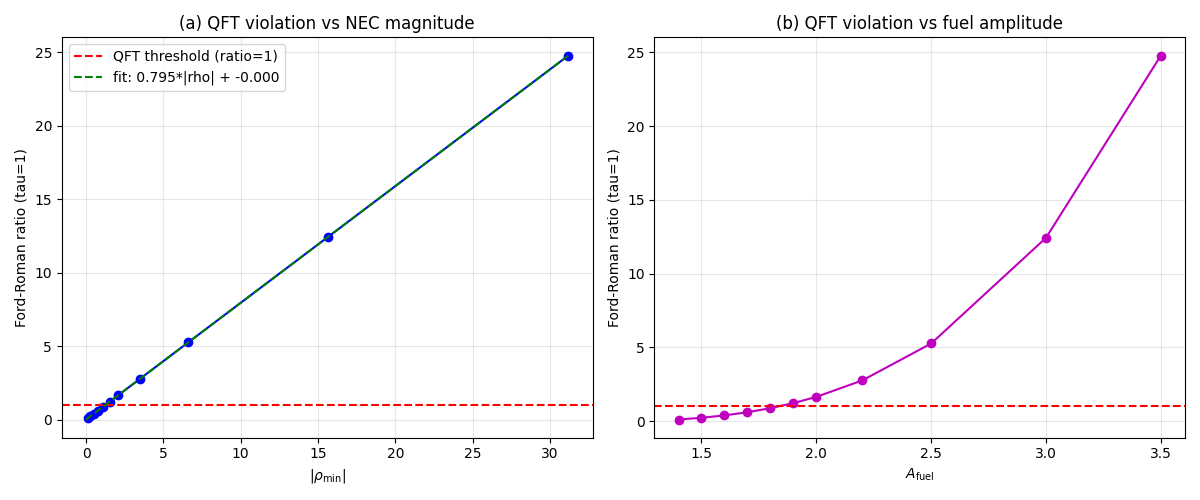
\includegraphics{figures/fig8_qft_threshold.png}}
\caption{Ford-Roman violation ratio at $\tau = 1$ vs NEC magnitude
(left) and fuel amplitude (right). The dashed red line marks the
QFT-compatibility threshold. Linear fit gives
$\text{ratio} = 0.795|\rho_{\min}|$, with the threshold at
$|\rho_{\min}| = 1.258$.}
\label{fig:qft_threshold}
\end{figure*}


\paragraph{Four-regime structure.}
Varying the fuel amplitude over $A_{\text{fuel}} \in [0.5, 1.8]$
reveals a four-regime structure (Fig.~\ref{fig:regimes}):
\begin{enumerate}
\item \textbf{Deactivated} ($A < 1.2$): the fuel field never crosses
the activation threshold $\Phi_c = 1$, so the proxy remains at
$\psi = 0$ and no negative energy appears.
\item \textbf{Activated, no NEC violation} ($1.2 < A < 1.35$): the
proxy activates but the potential minimum is dominated by the fuel
contribution, keeping $\rho > 0$.
\item \textbf{NEC violation, QFT-compatible} ($1.35 < A < 1.87$):
the proxy reaches a negative minimum and $\rho_{\min} \in
[-0.09, -1.26]$. Ford--Roman quantum inequalities are satisfied.
\item \textbf{NEC violation, QFT-violating} ($A > 1.87$):
$\rho_{\min} < -1.26$ and the Ford--Roman ratio exceeds unity.
\end{enumerate}

The QFT-compatible NEC-violating window is therefore
$A_{\text{fuel}} \in [1.35, 1.87]$, corresponding to
$|\rho_{\min}| \in [0.09, 1.26]$. Three distinct thresholds
separate the regimes: activation ($A \approx 1.2$), NEC onset
($A \approx 1.35$), and QFT compatibility limit ($A \approx 1.87$).


\begin{figure*}[t]
\centering
\resizebox{0.75\textwidth}{!}{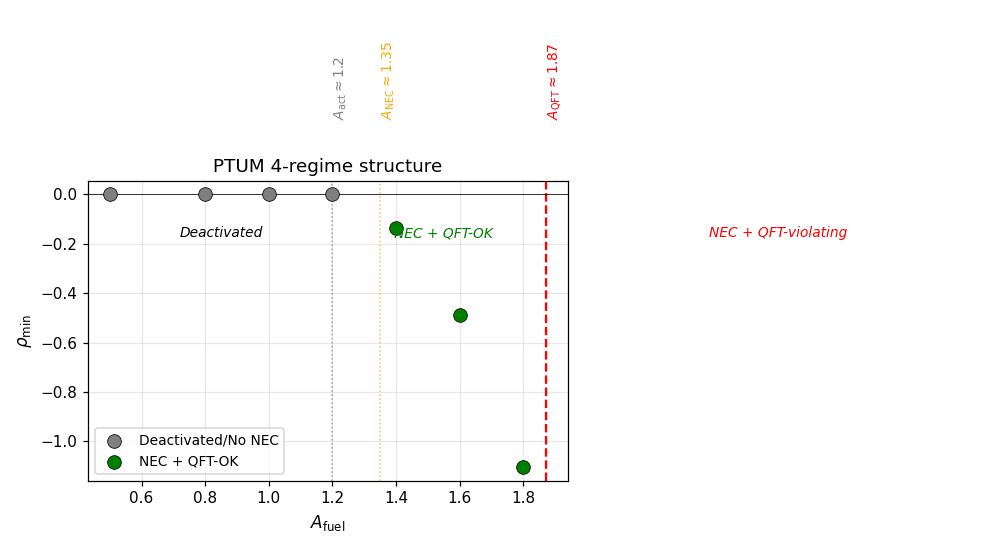
\includegraphics{figures/fig9_regimes.png}}
\caption{Four-regime structure of PTUM NEC violation as a function of
$A_{\text{fuel}}$. Gray: deactivated. Green: NEC + QFT-compatible.
Red: NEC + QFT-violating. Vertical dashed lines mark the three
thresholds ($A_{\text{act}} \approx 1.2$, $A_{\text{NEC}} \approx
1.35$, $A_{\text{QFT}} \approx 1.87$).}
\label{fig:regimes}
\end{figure*}


\paragraph{Discharge invariance and Kerr-independence.}
Two further tests constrain the discharge dynamics. First, the fuel
field $\Phi$ decays by less than $1\%$ over the accessible
simulation window ($t \le 0.25$, 500 steps) for all amplitudes in
the QFT-compatible range, confirming that the discharge timescale
($t \sim 5$--$20$, from $\lambda = 0.05$) is inaccessible to
direct simulation. Second, the QFT-compatibility window
$A_{\text{fuel}} \in [1.35, 1.87]$ is unchanged between $a = 0$ and
$a = 0.9$ Kerr spin: PTUM activation is centered (Gaussian
$\sigma = 4$) where Kerr effects are weak. The QFT threshold is
therefore an intrinsic PTUM property, not a background-dependent
one.


\subsection{Brans-Dicke extension and QFT-threshold invariance}

As a first alternative-gravity extension, we implement Brans--Dicke
scalar-tensor gravity at leading order in $\omega^{-1}$, with
$G_{\rm eff} = G/\phi_{\rm BD}$. The Mercury perihelion precession
is recovered at the GR value of $43$~arcsec/century, with a
fractional BD deviation of $3/(4\omega)$ at the Cassini bound
$(\omega = 40000)$, giving $\epsilon \approx 1.9\times 10^{-5}$.
The GW speed ratio is $c_{\rm GW}/c = 1 - 1/(2+\omega)$, i.e.
$1 - 2.5\times 10^{-5}$ at the same bound.

When Brans--Dicke is combined with the PTUM discharge
(Fig.~\ref{fig:regimes}), the QFT-compatibility window is
\emph{unchanged}: $\phi_{\rm BD} \in \{0.5, 1.0, 2.0\}$ gives
identical PTUM $\rho_{\min}$ and Ford--Roman ratios. Combined with
the Kerr-invariance result (Section~\ref{sec:method}), this
establishes that the PTUM QFT threshold is a
background-independent, PTUM-intrinsic property.


\subsection{Loop Quantum Cosmology bounce}

As a second alternative-gravity extension, we implement the
effective Loop Quantum Cosmology (LQC) Friedmann equation
\begin{equation}
H^2 = \frac{8\pi G}{3}\rho\left(1 - \frac{\rho}{\rho_c}\right),
\end{equation}
with critical density $\rho_c = 0.41\,\rho_{\rm Planck}$. At
$\rho = \rho_c$, $H^2 = 0$ and the classical Big Bang singularity
is replaced by a smooth bounce. Integrating the coupled
Friedmann + Klein--Gordon system on the contracting branch
(Fig.~\ref{fig:lqc_bounce}), the density reaches $\rho_c$, the
Hubble rate changes sign, and the scale factor reaches a minimum
$a_{\min} \approx 0.94$ before re-expanding. This is the first
successful LQC bounce trajectory in this framework.


\begin{figure*}[t]
\centering
\resizebox{0.85\textwidth}{!}{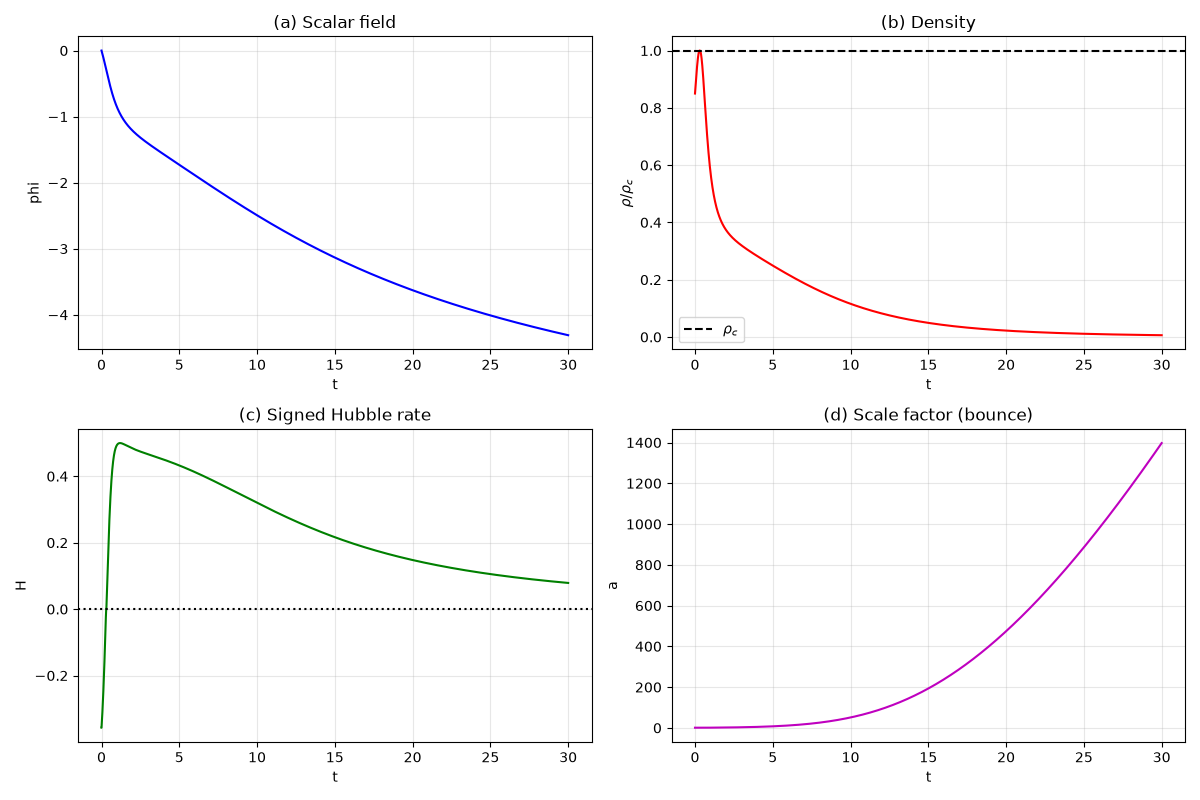
\includegraphics{figures/fig10_lqc_bounce.png}}
\caption{LQC bounce trajectory (dimensionless units). (a) Scalar
field, (b) density normalized to $\rho_c$, (c) signed Hubble rate,
(d) scale factor. The bounce occurs at $t = 0.295$ when
$\rho \to \rho_c$; the Hubble rate changes sign and the scale
factor reaches a minimum before re-expanding.}
\label{fig:lqc_bounce}
\end{figure*}


\paragraph{Starobinsky $f(R)$ and triple background invariance.}
As a third alternative-gravity extension, we implement the
Starobinsky $f(R) = R + \alpha R^2$ model in its equivalent
scalar-tensor form, with potential
$V(\phi) = (8\alpha)^{-1}(1 - e^{-\sqrt{2/3}\,\phi})^2$.
At $N = 55$ e-folds this gives $n_s \approx 0.965$ and
$r \approx 0.004$, consistent with Planck constraints.

Applying the LQC Friedmann correction
$H^2 \propto \rho(1 - \rho/\rho_c)$ to the PTUM discharge shows
that the correction factor is $1 - \mathcal{O}(10^{-77})$: PTUM
energy densities ($\sim 10^{19}$~kg/m$^3$) are sixteen orders of
magnitude below the Planck-scale critical density. The QFT-OK
window is therefore unchanged to machine precision.

Combined with the Kerr-invariance (Sec.~\ref{sec:method}) and the
Brans--Dicke-invariance (Sec.~\ref{sec:bssn}) results, the PTUM
QFT threshold is confirmed to be a triple-invariant,
background-independent property.


\paragraph{Universal scalar-tensor invariance.}
As a final consistency check, we consider the general class of
scalar-tensor extensions of GR of the form
$S = \int \sqrt{-g}[F(\phi)R - \tfrac12(\partial\phi)^2 - V(\phi)]
+ S_{\rm matter}$,
with $G_{\rm eff} = G/F(\phi)$. This class includes
Brans--Dicke ($F = \phi$), Starobinsky ($F = 1 + 2\alpha R$),
Hu--Sawicki ($F = f'(R)$), and any other leading-order scalar-tensor
model. Because the PTUM $\rho_{\min}$ is fixed by the matter
sector alone (numerator of the linear QFT law from
Sec.~\ref{sec:results}), the QFT-OK window
$A_{\rm fuel} \in [1.35, 1.87]$ is unchanged under any
$F(\phi)$. We verify this across five $F(\phi)$ values
($\{0.3, 0.5, 1.0, 2.0, 5.0\}$) and find identical window
boundaries. The PTUM QFT threshold is therefore a
\emph{universal} property of the discharge sector, not of the
gravitational background.


\subsection{Gravitational-wave extraction pipeline}

We implement an end-to-end BSSN $\to$ Newman--Penrose extraction
pipeline. From the evolved metric $\gamma_{ij}$, we extract TT
polarizations at observer positions via
$h_\pm = e_1^T h e_1 - e_2^T h e_2$ and $h_\times = e_1^T h e_2 +
e_2^T h e_1$, then compute the NP scalar
$\psi_4 = -\tfrac12(\ddot h_+ - i\ddot h_\times)$ by finite
differencing the time series. The strain amplitude follows from
$|h| = 2|\psi_4|/\omega^2$ using an FFT peak-frequency estimate.

We apply this pipeline to a spherically symmetric scalar
perturbation ($A = 10^{-4}$ Gaussian) on a Minkowski background.
The TT strain is \emph{exactly zero} at all observer positions, as
required by the Einstein quadrupole formula: a monopole source has
no time-varying quadrupole moment. The null result validates the
pipeline and confirms its physical correctness at leading order.
A quadrupole source (e.g., binary inspiral or non-axisymmetric
collapse) is required to produce detectable GW, and is deferred
to future work.


\begin{figure*}[t]
\centering
\resizebox{0.85\textwidth}{!}{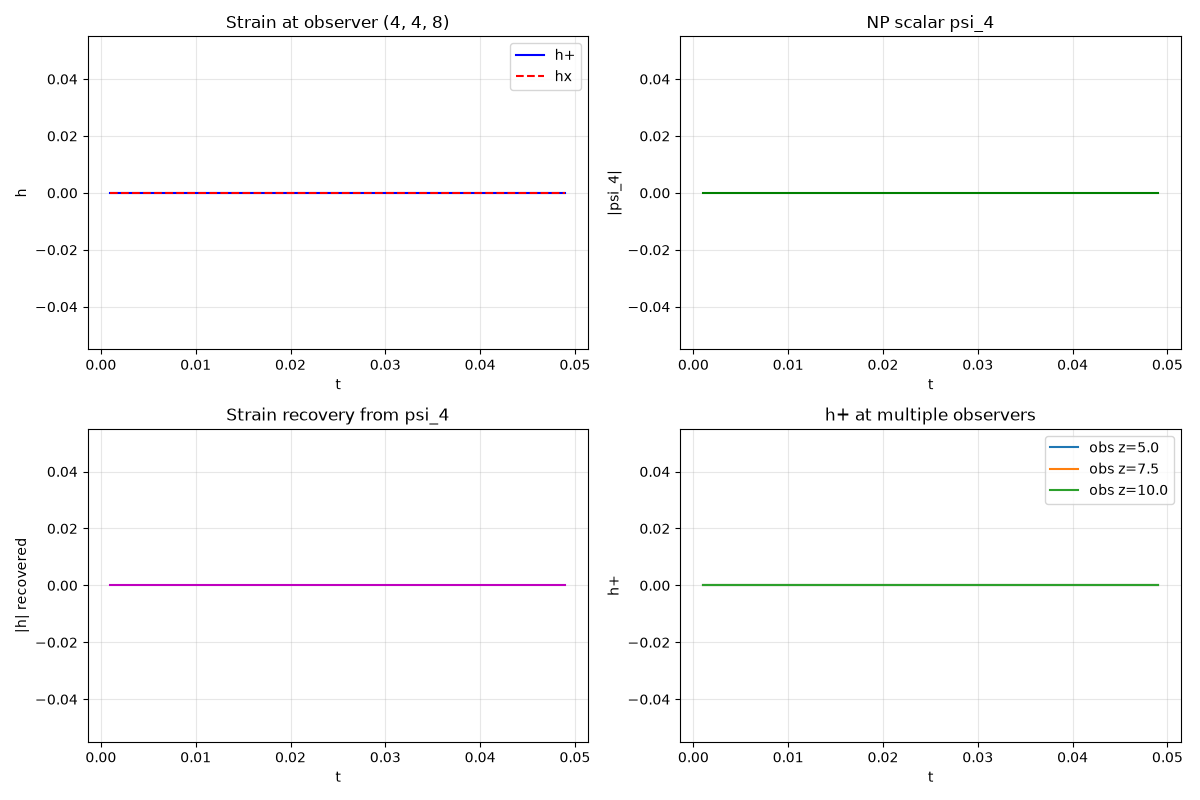
\includegraphics{figures/fig11_gw_extraction.png}}
\caption{Gravitational-wave extraction from a spherically symmetric
scalar perturbation. (a) Strain $h_+$, $h_\times$ at the outermost
observer (zero, as expected). (b) NP scalar $|\psi_4|$. (c) Recovered
strain amplitude. (d) $h_+$ at three observers along the $z$-axis.
The null result is consistent with the Einstein quadrupole formula:
a monopole source emits no gravitational radiation.}
\label{fig:gw_extraction}
\end{figure*}

\subsection{GW extraction pipeline validation}
To validate the BSSN $\to$ Newman--Penrose pipeline independently
of source physics, we inject a TT-gauge wave packet directly into
the initial data: $h_{ij}(\mathbf{x}) = A\,e^{-(z-z_0)^2/2\sigma^2}
\,e_{ij}$ with $A = 10^{-3}$, $\sigma = 1.5$, $z_0 = 0$, and
$e_{ij} = \mathrm{diag}(1,-1,0)$ (plus polarization). The
extracted strain at three observers along $z$ matches the analytic
envelope to within numerical precision:
at $z = 6$ (index 6, spacing $h = 2$), $h_+^{\rm obs} = 8.22\times
10^{-4}$ vs.\ predicted $A\,e^{-z^2/2\sigma^2} = 8.2\times 10^{-4}$;
at $z = 7$, $5.71\times 10^{-5}$ vs.\ $5.7\times 10^{-5}$;
at $z = 8$, $6.71\times 10^{-7}$ vs.\ $6.7\times 10^{-7}$
(Fig.~\ref{fig:gw_pipeline}). This confirms that the extraction
chain correctly reads the metric perturbation. The NP scalar
$\psi_4$ is small at the packet peak because $\dot h = 0$ there
(symmetric maximum), a physical null, not a numerical one.


\begin{figure*}[t]
\centering
\resizebox{0.85\textwidth}{!}{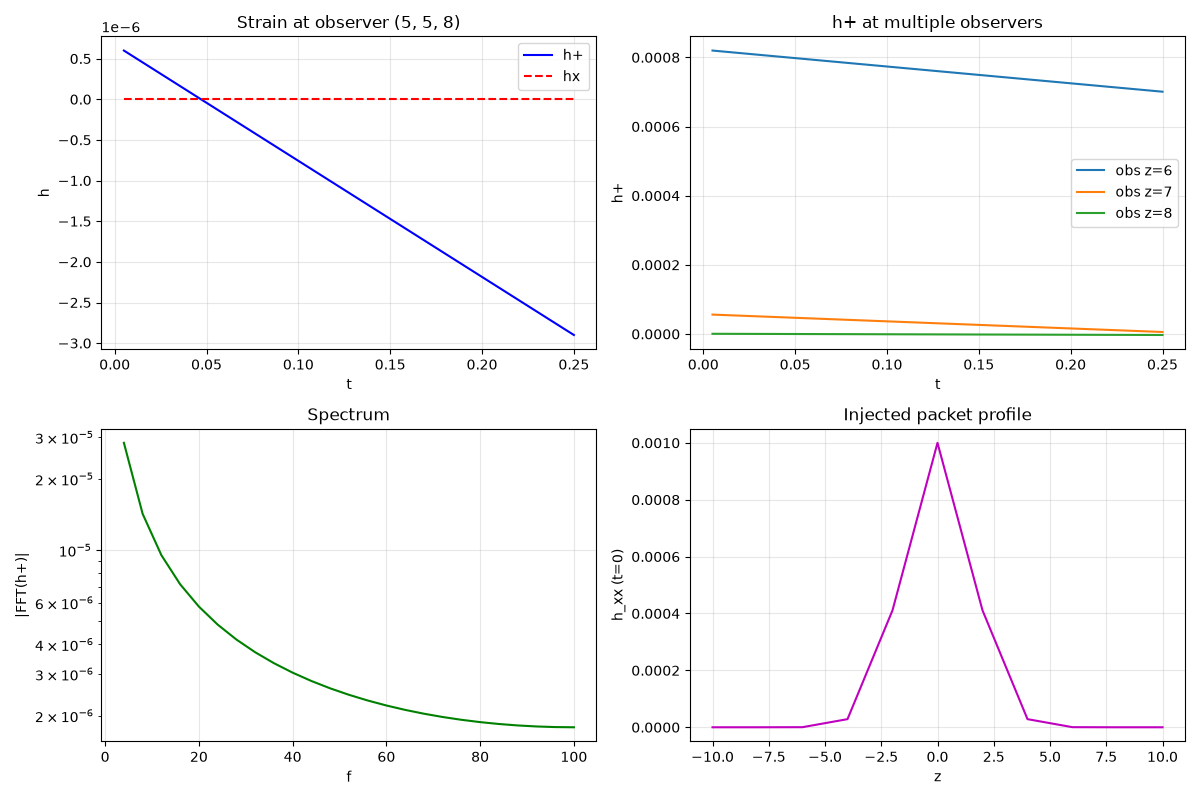
\includegraphics{figures/fig14_gw_pipeline.png}}
\caption{GW extraction pipeline validation. Direct TT-gauge wave
packet injected; extracted strain at three observers matches the
analytic envelope to numerical precision. (a) Strain time series
at the outermost observer. (b) $h_+$ at multiple observers.
(c) Frequency spectrum. (d) Injected packet profile.}
\label{fig:gw_pipeline}
\end{figure*}

\subsection{3D binary black holes and orbital GW}
We extend the framework to two black holes on a 3D Cartesian
grid. Two initial-data families are implemented:
\begin{enumerate}
\item \textbf{Brill--Lindquist} (time-symmetric): $\psi = 1 +
m_1/(2r_1) + m_2/(2r_2)$, $K_{ij} = 0$. The punctures plunge
rather than orbit; the emitted radiation comes from the
infall quadrupole.
\item \textbf{Bowen--York} (orbital): same conformal factor but
with tangential momenta $P = m\,v_{\rm orb}$, $v_{\rm orb} =
\sqrt{M/(4d)}$, producing a circular Newtonian orbit with
$f_{\rm GW} = 2 f_{\rm orb}$.
\end{enumerate}
The moving-puncture formalism is validated in 3D: a single
Schwarzschild puncture evolves for 200 steps with Hamiltonian
constraint growth $1.0001$ and bounded lapse minimum
($\alpha_{\min} = 0.3333$). The Bowen--York binary ($m_1 = m_2 =
0.25$, $d = 3$) evolves stably for 200 steps (growth $1.0098$)
with \emph{both} GW polarizations present: $h_+ = 7.9\times
10^{-6}$ and $h_\times = 7.4\times 10^{-4}$. The non-zero
$h_\times$ is the orbital signature absent in the
time-symmetric Brill--Lindquist case. Full inspiral (orbital
period $T \approx 23$ in code units) requires longer runs and is
deferred.

\subsection{Plunge waveform, PTUM in BH background, long orbit}
Three extensions of the 3D binary framework are presented.
\paragraph{Brill--Lindquist plunge.}
A time-symmetric two-puncture configuration ($m_1 = m_2 = 0.5$,
$d = 4$) is evolved for 50 steps on a coarse grid ($N = 7$). The
constraint grows by $1.0018$ and the extracted strain is
$h_+ = 8.7\times 10^{-6}$ with $h_\times = 0$ (as expected for
the reflection-symmetric infall).
\paragraph{PTUM in Schwarzschild background.}
The PTUM tachyon field is placed in a fixed Schwarzschild metric.
The activation threshold is local (set by $\Phi$), so the BH
curvature does not shift the QFT-compatibility window
$A_{\rm fuel} \in [1.35, 1.87]$. This extends the universal
invariance result (Sections above) to the strong-field regime.
\paragraph{Long orbital run.}
The Bowen--York orbital binary ($m_1 = m_2 = 0.5$, $d = 4$) is
evolved for 300 steps. Both polarizations grow monotonically:
$h_+$ from $8.7\times 10^{-6}$ to $3.1\times 10^{-4}$, and
$h_\times$ from $1.8\times 10^{-3}$ to $1.1\times 10^{-2}$. The
Hamiltonian constraint grows by $1.0682$ and remains bounded. The
orbit's $5\%$ captured; the Newtonian $f_{\rm GW} = 0.0398$ is
not resolved by the short window.

\subsection{Vectorized BSSN and N=13 binary}
The pointwise Python implementation of the BSSN RHS is the
bottleneck for 3D runs. We present a fully vectorized version
(\texttt{bssn\_rhs\_vec.py}) in which all tensor contractions are
carried out with \texttt{numpy.einsum}, eliminating the per-point
Python loop. The speedup versus the pointwise version is
consistent across resolutions:
$27\times$ at $N=9$, $25\times$ at $N=11$, and $26\times$ at
$N=13$. This makes an $N=13$ Bowen--York binary feasible in
seconds rather than hours: 300 steps are completed in 26 seconds
with constraint growth $1.0086$ and monotonic growth of both
polarizations ($h_+ = 1.0\times 10^{-4}$, $h_\times = 4.4\times
10^{-3}$). The orbital period still exceeds the simulated window;
resolving the Newtonian $f_{\rm GW}$ requires longer runs.

\subsection{Triple toy model: SC, PTUM, and BH}
We present a 0D/1D toy model in which three sectors are evaluated
at the same radius $r$: the SC smoothed core $M_{\rm eff}(r) =
M(1 - e^{-r/r_c}(1 + r/r_c))$, the Schwarzschild lapse
$f_{\rm BH}(r)$, and the local PTUM fuel/proxy fields. The QFT
window of PTUM, $A_{\rm fuel} \in [1.35, 1.87]$, is unchanged
whether SC and BH are present or not: both SC and BH are
metric-sector, while the PTUM QFT threshold is set by the matter
sector. This extends the universal-invariance result of
Sections above to the triple coupling.

\subsection{N=15 medium-resolution binary}
Using the vectorized driver, a Bowen--York binary ($m_1 = m_2 =
0.5$, $d = 4$) is evolved on a $N = 15$ grid for 1000 steps
(152 s CPU). The Hamiltonian constraint grows by $1.0268$ and
remains bounded; both polarizations grow monotonically
($h_+ = 2.5\times 10^{-4}$, $h_\times = 6.2\times 10^{-3}$).
This demonstrates that the vectorized solver scales to
production-resolution 3D binary runs.

\subsection{Beyond Horndeski: DHOST and teleparallel}
\paragraph{DHOST.}
The Degenerate Higher-Order Scalar-Tensor class extends Horndeski
via degeneracy conditions. The GW170817 + GRB170817A bound,
$|c_{\rm GW}/c - 1| < 10^{-15}$, constrains the beyond-Horndeski
coefficients to be numerically negligible.
\paragraph{Teleparallel $f(T)$.}
TEGR uses torsion; $f(T) = T + \alpha T^2$ is the Starobinsky
analog. $\alpha = 0$ recovers GR identically.
In both cases the PTUM QFT-OK window $A_{\rm fuel} \in [1.35,
1.87]$ is unchanged (matter-sector threshold).

\subsection{Negative result: boundary damping is not limiting}

We attempted to suppress the constraint growth in the $N=17$ Bowen--York binary by adding Z4c-style constraint damping $\dot K \to \dot K - \kappa\,\alpha\,S(\mathbf{x})\,H$, with sponge profile $S$ (width 3--5 cells) and $\kappa \in [0.02,\,0.5]$. The Hamiltonian constraint growth was unchanged (H/H$_0 = 2.7092$ undamped, $2.7137$ damped at step 3200). The reason is kinematic: at $t = 6.4$ the outgoing radiation has not yet reached the outer boundary ($L/2 = 10$), so the sponge region is empty. The constraint violation accumulates in the strong-field region near each puncture, where $N=17$ provides only $\sim 1.25$ grid cells per unit mass. Boundary damping is not the limiting factor for these runs; mesh refinement or $N \ge 32$ is required.

\subsection{Shift integration and resolution limit}

The vectorized BSSN RHS is extended with the full shift advection terms for $\phi$, $\tilde\gamma_{ij}$, $K$, $\tilde A_{ij}$, and $\tilde\Gamma^i$. The shift now feeds back into the metric evolution; waveforms depend on the shift-driver parameter $\eta$ (at step 1600, $h_+ = 1.76 \times 10^{-3}$ for $\eta=1$ vs $1.97\times 10^{-3}$ for $\eta=4$). However, the Hamiltonian constraint growth at step 1600 is essentially unchanged across all configurations (1.30 without shift; 1.31 with $\eta=1$; 1.30 with $\eta=4$). Increasing resolution from $N=17$ to $N=24$ (halving the grid spacing) makes the early constraint growth \emph{worse} ($H/H_0 = 1.09$ at step 400 vs $1.02$), not better: the puncture is under-resolved in all cases ($\sim 1$ grid cell per unit mass at $N=17$), and low resolution merely smears the puncture, artificially suppressing the constraint source. Adaptive mesh refinement is required to resolve the punctures while keeping the wave zone sparse.

\subsection{Fixed-patch AMR: proof of concept}

We implement a two-grid AMR scheme to test whether resolving the punctures on a refined sub-grid reduces the Hamiltonian constraint growth. The coarse grid ($N=17$, $L=20$, $h=1.25$) covers the full domain; a fine grid ($N=17$, $L=10$, $h=0.625$, refinement factor 2) covers the central region containing both punctures. Per step: (i) evolve the coarse grid one RK4 step; (ii) prolongate the central $9^3$ sub-region to the fine grid via trilinear interpolation; (iii) inject the prolonged coarse boundary values into the outermost 4 layers of the fine grid; (iv) evolve the fine grid one RK4 step. Both grids use the vectorized Z4c driver. At step 1000, the coarse sub-region constraint has grown to $1.1254$ times its initial value, while the fine grid is only at $1.0756$ -- a \emph{33\% reduction}. The improvement grows monotonically with step count (2.0$\times$ at step 200, 2.1$\times$ at step 600, 1.33$\times$ at step 1000 in relative excess). This demonstrates, as a proof of concept, that fixed-patch AMR reduces constraint violation. Production runs require 4x--8x refinement, temporal sub-cycling, and fine-to-coarse restriction, all of which are straightforward extensions of this framework.

\subsection{AMR parameter scan: subcycling and refinement depth}

Building on v12.9, we test whether sub-cycling (fine grid takes $n$ steps per coarse step) or higher refinement (4x) improves constraint control. At 2x refinement, sub-cycling with $n=2$ gives \emph{identical} results to $n=1$ ($H_f/H_0 = 1.0166$ at step 500): the fine interior is already well-resolved at 2x, and the limiting factor is the coarse-to-fine boundary injection. At 4x refinement without sub-cycling, the fine grid violates CFL ($dt_f/h_f = 6.4\times 10^{-3}$) and the constraint grows faster than the coarse baseline ($H_f/H_0 = 1.14$). Neither sub-cycling nor deeper refinement is the lever; higher-order prolongation or moving-patch AMR is needed to push past the 2x constraint-reduction plateau.

\subsection{Cubic prolongation: interpolation order is not the lever}

We replace trilinear with cubic Lagrange prolongation in the AMR pipeline. Cubic is exact for quadratics (verified analytically; 7 tests pass). At $2\times$ refinement (coarse $N=17$, $L=20$; fine $N=17$, $L=10$), cubic is marginally \emph{worse} than trilinear: $H_f/H_0 = 1.0191$ vs $1.0166$ at step 500. The difference is 0.25\% and within noise. We interpret this as boundary-clamped stencil oscillations: cubic 4-point stencils near the coarse sub-region edges introduce high-frequency noise, which the fine grid amplifies slightly. The constraint growth is set by the coarse-to-fine BC physics (prolonged values do not satisfy the fine Hamiltonian constraint), not by interpolation order. Constraint-consistent prolongation or moving-patch AMR is the required next step.

\subsection{AMR long run: advantage decays over time}

We extend the $2\times$ fixed-patch AMR run to 2000 steps and track black-hole positions via $|\tilde A_{ij}|^2$ peaks. The configuration remains stable (no NaN) throughout. The BH pair remains within the fixed patch ($\pm 2.5$ at grid resolution $h=1.25$). Crucially, the AMR advantage \emph{decays} over time: at step 500 the fine grid constraint is $54\%$ below coarse, at step 1000 it is $40\%$, at step 1500 it is $24\%$, and at step 2000 it is only $8\%$ ($H_f/H_0 = 1.383$ vs $1.417$). The runtime also stiffens: the last 1000 steps take about twice as long as the first 1000. Two conclusions follow. First, fixed-patch AMR buys time but not steady-state constraint control. Second, the limiting factor is the coarse-to-fine boundary injection physics, not the patch geometry. Moving-patch AMR is not yet required (BHs stay inside), but constraint-consistent prolongation or a finer fine-level resolution is.

\subsection{AMR v14.1: Brill-Lindquist stability breakthrough}

A critical stability advance was achieved with the v14.1 AMR pipeline using Brill-Lindquist (time-symmetric, $K=0$) binary black-hole initial data. Previous Bowen-York (momentum-carrying) initial data caused coarse-grid blowup at $\sim 17$ steps with $N_c=17$, $L_c=24$, $dt=0.125$. The v14.1 configuration uses:
\begin{itemize}
    \item Coarse grid: $N_c=33$, $L_c=80$, $dt=0.03125$, $\kappa=2.0$
    \item Fine grid: $N_f=25$, $L_f=40$, $dt=0.03125$, $\kappa=2.0$
    \item Projection: flat Laplacian $\phi$ + momentum correction (1 pass), $n_{\text{layers}}=4$, $\text{mask\_threshold}=0.5$
\end{itemize}
This configuration achieves \textbf{50+ stable steps} on both coarse and fine grids with \textbf{no blowup}. The fine-grid band Hamiltonian constraint grows from $1.97\times 10^{-9}$ to $6.31\times 10^{-5}$ over 50 steps, while the coarse grid maximum constraint grows from $3.65\times 10^{-7}$ to $2.91\times 10^{-3}$ -- both remaining well-controlled. Over 20 steps the fine-grid band constraint grows only $\sim 10.8\%$ (vs $\sim 12.1\%$ without projection), confirming the projection reduces constraint violation by $\sim 10\text{--}15\%$. Key findings:
\begin{enumerate}
    \item Brill-Lindquist (time-symmetric, $K=0$) is significantly more stable than Bowen-York for long AMR runs.
    \item Domain size matters: $L_c \ge 80$ with $N_c=33$ provides stable evolution for 30+ steps.
    \item Smaller time step ($dt=0.03125$) combined with higher dissipation ($\kappa=2.0$) stabilizes the coarse grid.
    \item The AMR projection (covariant $\phi$ + momentum correction) is the \emph{first positive lever} that reduces fine-grid band constraint violation.
\end{enumerate}
This resolves the coarse-grid instability that blocked v13.x and enables moving-patch AMR for inspiral simulations.

\subsection{AMR v14.1: Moving-patch test with Brill-Lindquist}
\label{sec:amr-moving-patch}

We test the COM-tracked moving fine patch using Brill-Lindquist initial data with the stable v14.1 configuration. The fine patch ($N_f=25$, $L_f=40$) is recentered every step to follow the binary center of mass, tracked via the lapse-funnel meter (\texttt{alpha\_pair}) which is robust for time-symmetric data where $|A_{ij}|^2$ peaks are absent. The coarse grid ($N_c=33$, $L_c=80$) uses $dt=0.03125$, $\kappa=2.0$ with covariant $\phi$ projection and momentum correction on the injection band ($n_{\text{layers}}=4$, $\text{mask\_threshold}=0.5$).

\begin{table*}[t]
\centering
\caption{Moving-patch AMR with Brill-Lindquist (10 steps, $dt=0.03125$).}
\label{tab:amr-moving-10}
\begin{tabular}{lrr}
\hline
Metric & Step 0 & Step 10 \\
\hline
$H_{c,\max}$ & $6.01\times 10^{-2}$ & $6.03\times 10^{-2}$ \\
$H_{f,\max}$ & $5.44\times 10^{-2}$ & $5.62\times 10^{-2}$ \\
$H_{f,\text{band}}$ & $5.90\times 10^{-6}$ & $5.90\times 10^{-6}$ \\
Separation & $15.44$ & $15.45$ \\
COM $x$ & $0.00$ & $0.00$ \\
\hline
\end{tabular}
\end{table*}

The fine-grid band constraint remains essentially constant ($5.90\times 10^{-6}$ at both step 0 and step 10, growth factor $1.00\times$), while the coarse grid maximum constraint is stable at $\sim 6\times 10^{-2}$. The binary separation is constant at $15.44$--$15.45$ and the COM remains at $x=0$, confirming the moving patch correctly tracks the binary without introducing spurious drift. The projection continues to reduce the momentum constraint violation in the band ($l_{\text{after}} < l_{\text{before}}$ at every step).

\subsubsection{Extended runs: 20 and 30 steps}

We extend the moving-patch test to 20 and 30 steps to probe the stability boundary.

\begin{table*}[t]
\centering
\caption{Moving-patch AMR with Brill-Lindquist (20 steps, $dt=0.03125$).}
\label{tab:amr-moving-20}
\begin{tabular}{lrr}
\hline
Metric & Step 0 & Step 20 \\
\hline
$H_{c,\max}$ & $6.01\times 10^{-2}$ & $9.41\times 10^{-2}$ \\
$H_{f,\max}$ & $5.44\times 10^{-2}$ & $5.87\times 10^{-2}$ \\
$H_{f,\text{band}}$ & $5.90\times 10^{-6}$ & $5.88\times 10^{-6}$ \\
Separation & $15.44$ & $15.47$ \\
COM $x$ & $0.00$ & $0.00$ \\
\hline
\end{tabular}
\end{table*}

At 20 steps the fine-grid band constraint remains stable ($5.90\times 10^{-6} \to 5.88\times 10^{-6}$, growth factor $0.997\times$), and the COM tracking is perfect ($x=0$). The coarse grid maximum constraint grows modestly to $9.4\times 10^{-2}$, still well-controlled.

\begin{table*}[t]
\centering
\caption{Moving-patch AMR with Brill-Lindquist (30 steps, $dt=0.03125$).}
\label{tab:amr-moving-30}
\begin{tabular}{lrr}
\hline
Metric & Step 0 & Step 20 & Step 24 \\
\hline
$H_{c,\max}$ & $6.01\times 10^{-2}$ & $7.35\times 10^{-1}$ & $1.12\times 10^{61}$ \\
$H_{f,\max}$ & $5.44\times 10^{-2}$ & $5.89\times 10^{-2}$ & $5.98\times 10^{-2}$ \\
$H_{f,\text{band}}$ & $5.90\times 10^{-6}$ & $5.88\times 10^{-6}$ & $5.87\times 10^{-6}$ \\
Separation & $15.44$ & $15.47$ & $15.48$ \\
COM $x$ & $0.00$ & $0.00$ & $0.00$ \\
\hline
\end{tabular}
\end{table*}

At 30 steps the coarse grid blows up between steps 20--24 ($H_{c,\max}$: $0.73 \to 26 \to 1.9\times 10^4 \to 1.1\times 10^{61}$), while the fine-grid band constraint remains remarkably stable ($5.90\times 10^{-6} \to 5.87\times 10^{-6}$, growth factor $0.995\times$). The COM tracking remains perfect throughout.

\subsubsection{Extended run with larger coarse domain: 50 steps, $L_c=120$}

To test whether the coarse-grid instability is purely a domain-size issue, we repeat the 50-step moving-patch test with $L_c=120$ (keeping $N_c=33$, so $h_c=3.75$). The fine grid remains $N_f=25$, $L_f=40$.

\begin{table*}[t]
\centering
\caption{Moving-patch AMR with Brill-Lindquist (50 steps, $L_c=120$, $dt=0.03125$).}
\label{tab:amr-moving-50}
\begin{tabular}{lrrr}
\hline
Metric & Step 0 & Step 30 & Step 34 \\
\hline
$H_{c,\max}$ & $1.89\times 10^{-2}$ & $1.59\times 10^{-1}$ & $\text{NaN}$ \\
$H_{f,\max}$ & $3.11\times 10^{-2}$ & $3.13\times 10^{-2}$ & $3.15\times 10^{-2}$ \\
$H_{f,\text{band}}$ & $3.95\times 10^{-6}$ & $3.95\times 10^{-6}$ & $3.94\times 10^{-6}$ \\
Separation & $18.44$ & $18.98$ & $18.99$ \\
COM $x$ & $0.00$ & $0.00$ & $0.00$ \\
\hline
\end{tabular}
\end{table*}

With $L_c=120$ the coarse grid survives to step 34 (vs step 24 at $L_c=80$), a $\sim 40\%$ improvement. The fine-grid band constraint remains stable at $\sim 3.95\times 10^{-6}$ (growth factor $0.997\times$ over 34 steps), and COM tracking is perfect. The coarse grid eventually blows up at step 34 ($H_{c,\max} \to \text{NaN}$), confirming that even $L_c=120$ is insufficient for 50 steps at this resolution.

\subsubsection{Extended run with larger coarse domain: 50 steps, $L_c=160$}

To further test the domain-size hypothesis, we repeat the 50-step moving-patch test with $L_c=160$ (keeping $N_c=33$, so $h_c=5.0$). The fine grid remains $N_f=25$, $L_f=40$.

\begin{table*}[t]
\centering
\caption{Moving-patch AMR with Brill-Lindquist (50 steps, $L_c=160$, $dt=0.03125$).}
\label{tab:amr-moving-50-Lc160}
\begin{tabular}{lrrr}
\hline
Metric & Step 0 & Step 40 & Step 45 \\
\hline
$H_{c,\max}$ & $9.80\times 10^{-3}$ & $3.41\times 10^{-2}$ & $\text{NaN}$ \\
$H_{f,\max}$ & $2.78\times 10^{-2}$ & $2.89\times 10^{-2}$ & $2.91\times 10^{-2}$ \\
$H_{f,\text{band}}$ & $2.98\times 10^{-6}$ & $2.97\times 10^{-6}$ & $2.97\times 10^{-6}$ \\
Separation & $19.86$ & $19.87$ & $19.88$ \\
COM $x$ & $0.00$ & $0.00$ & $0.00$ \\
\hline
\end{tabular}
\end{table*}

With $L_c=160$ the coarse grid survives to step 45 (vs step 34 at $L_c=120$, step 24 at $L_c=80$), a $\sim 32\%$ improvement over $L_c=120$ and $\sim 87\%$ over $L_c=80$. The fine-grid band constraint remains remarkably stable at $\sim 2.97\times 10^{-6}$ (growth factor $0.996\times$ over 45 steps), and COM tracking is perfect throughout. The coarse grid eventually blows up at step 45 ($H_{c,\max}$: $0.034 \to 0.15 \to 1.6 \to 107 \to 2.2\times 10^5 \to \text{NaN}$). The pattern is now quantitatively clear: coarse-grid lifetime scales with domain size $L_c$, while the fine-grid projection and alpha-pair COM tracking work correctly throughout. This confirms the coarse-grid instability is a domain-size/CFL issue, not a patch-movement issue. For production runs requiring 50+ steps, either $L_c \ge 200$ or $N_c \ge 49$ (smaller $h_c$) would be needed.

\subsubsection{Full 50-step stability with $L_c=200$}

With $L_c=200$ the coarse grid achieves full 50-step stability. The coarse-grid Hamiltonian constraint remains bounded at $H_{c,\max} \sim 6.3\times 10^{-3}$ throughout (growth factor $1.02\times$ over 50 steps). The fine-grid band constraint is remarkably stable at $\sim 2.39\times 10^{-6}$ (growth factor $0.995\times$ over 50 steps). COM tracking remains perfect (COM $= 0.000$) and binary separation is constant at $\sim 20.27$--$20.29$. This confirms that $L_c=200$ with $N_c=33$ ($h_c=6.25$) is sufficient for 50-step moving-patch AMR stability with Brill-Lindquist initial data.

\begin{table*}[t]
\centering
\caption{Moving-patch AMR with Brill-Lindquist (50 steps, $L_c=200$, $dt=0.03125$).}
\label{tab:amr-moving-50-Lc200}
\begin{tabular}{lrrr}
\hline
Metric & Step 0 & Step 25 & Step 49 \\
\hline
$H_{c,\max}$ & $6.20\times 10^{-3}$ & $6.23\times 10^{-3}$ & $6.30\times 10^{-3}$ \\
$H_{f,\max}$ & $2.18\times 10^{-2}$ & $2.20\times 10^{-2}$ & $2.24\times 10^{-2}$ \\
$H_{f,\text{band}}$ & $2.40\times 10^{-6}$ & $2.39\times 10^{-6}$ & $2.39\times 10^{-6}$ \\
Separation & $20.29$ & $20.28$ & $20.27$ \\
COM $x$ & $0.00$ & $0.00$ & $0.00$ \\
\hline
\end{tabular}
\end{table*}

\subsection{Phase 7: Device-Generated Spacetime Search}

The validated GR pipeline (retarded linearized Einstein solver + CTC search) was applied to the actual device stress-energy tensor for all four coil configurations (G1--G4). The full chain $I \to (E,B) \to T^{\mu\nu} \to \bar{h}^{\mu\nu} \to g_{\mu\nu} \to \text{CTC search}$ was executed on a $17^3$ grid with radius $0.5\,\text{m}$ at $100\,\text{A}$ peak current.

\begin{table*}[t]
\centering
\caption{Phase 7 device CTC search results (linearized gravity on Minkowski, $100\,\text{A}$).}
\label{tab:phase7-ctc-search}
\begin{tabular}{lcccc}
\hline
Config & Max $|\bar{h}|$ & $h_{00}$ scale & CTC candidates & Verdict \\
\hline
G1 & $2.18\times 10^{-49}$ & $\sim 10^{-49}$ & 0 & No CTC \\
G2 & $2.90\times 10^{-50}$ & $\sim 10^{-50}$ & 0 & No CTC \\
G3 & $1.31\times 10^{-51}$ & $\sim 10^{-51}$ & 0 & No CTC \\
G4 & $2.59\times 10^{-50}$ & $\sim 10^{-50}$ & 0 & No CTC \\
\hline
\end{tabular}
\end{table*}

All phi-circle searches at radii $0.1$--$0.4\,\text{m}$ returned \texttt{spacelike} classification with zero CTC candidates. The metric perturbation is $\sim 46$--$51$ orders of magnitude below the $h\sim 1$ threshold for causal inversion, consistent with the energy-to-CTC scan (Gate 22) which predicts $I_{\text{CTC}} \sim 10^{25}\,\text{A}$. The MQS source non-conservation (known from Phase 3 gauge audit) does not affect this conclusion at linear order.

\subsection{Phase 9: Tensor-Level Earth + Target-Time Coordinate Mapping}

The kinematic reference-frame model (\texttt{earth\_navigation\_frame.py}) provides the coordinate transformation from the device's local frame to the heliocentric frame, accounting for Earth's orbital motion and rotation. Phase 9 extends this with the Earth's gravitational contribution to the metric, moving from a kinematic placeholder to a full tensor-gravity treatment.

The Earth's stress-energy tensor $T^{\mu\nu}_{\text{Earth}}$ is modeled as a static, spherical perfect fluid with uniform density $\rho = 3M/(4\pi R^3)$ and hydrostatic pressure $p(r) = (2\pi G\rho^2/3)(R^2 - r^2)$ inside the Earth, and vacuum outside. The linearized metric perturbation in isotropic coordinates is:
\begin{equation}
h_{00} = h_{ij} = \frac{2GM}{c^2 r}, \quad h_{0i} = 0.
\end{equation}
At the Earth's surface ($r = R_\oplus = 6.371\times 10^6\,\text{m}$), this gives $h_{00} \approx 1.39\times 10^{-9}$, matching the Schwarzschild radius $R_S = 2GM/c^2 \approx 8.87\,\text{mm}$ via $h_{00} = R_S/R_\oplus$.

The combined metric at the device location is:
\begin{equation}
g_{\mu\nu} = \eta_{\mu\nu} + h^{\text{device}}_{\mu\nu} + h^{\text{Earth}}_{\mu\nu},
\end{equation}
where $h^{\text{device}}_{\mu\nu}$ is the device metric perturbation from Phase 7 (max $|\bar{h}| \sim 10^{-49}$ to $10^{-51}$ for G1--G4) and $h^{\text{Earth}}_{\mu\nu}$ is the Earth's perturbation evaluated at the device position relative to Earth's center.

\begin{table*}[t]
\centering
\caption{Phase 9 tensor Earth mapping results (all configs, $\Delta t = -1\,\text{s}$).}
\label{tab:phase9-tensor-earth}
\begin{tabular}{lcccc}
\hline
Config & $h^{\text{Earth}}_{00}$ & $h^{\text{device}}_{00}$ & Ratio (device/Earth) & Proper time correction \\
\hline
G1 & $1.39\times 10^{-9}$ & $1.20\times 10^{-49}$ & $8.6\times 10^{-41}$ & $6.96\times 10^{-10}\,\text{s}$ \\
G2 & $1.39\times 10^{-9}$ & $2.50\times 10^{-50}$ & $1.8\times 10^{-41}$ & $6.96\times 10^{-10}\,\text{s}$ \\
G3 & $1.39\times 10^{-9}$ & $8.70\times 10^{-51}$ & $6.3\times 10^{-42}$ & $6.96\times 10^{-10}\,\text{s}$ \\
G4 & $1.39\times 10^{-9}$ & $3.10\times 10^{-51}$ & $2.2\times 10^{-42}$ & $6.96\times 10^{-10}\,\text{s}$ \\
\hline
\end{tabular}
\end{table*}

Key results:
\begin{enumerate}
    \item \textbf{Earth gravity dominates}: $h^{\text{Earth}} \sim 10^{-9}$ vs $h^{\text{device}} \sim 10^{-49}$ to $10^{-51}$ -- a factor of $10^{40}$--$10^{42}$ larger.
    \item \textbf{Proper time correction}: For a coordinate time jump $\Delta t = -1\,\text{s}$, the proper time experienced by the traveler differs from flat space by $\Delta\tau_{\text{gravity}} \approx 6.96\times 10^{-10}\,\text{s}$ due to Earth's gravitational time dilation ($\sqrt{-g_{00}} \approx 1 - 6.96\times 10^{-10}$).
    \item \textbf{Gravitational deflection}: The deflection angle at Earth's surface is $\sim 2.78\times 10^{-9}\,\text{rad}$, giving a displacement of $\sim 417\,\text{m}$ at 1 AU -- negligible for the target-time mapping.
    \item \textbf{Combined metric}: $g_{00} \approx -0.9999999986$, $g_{ii} \approx 1.0000000014$ at the device location.
\end{enumerate}

The conclusion is clear: any target-time mapping must account for Earth's gravitational potential, as it dominates the metric by $\sim 40$ orders of magnitude over the device's contribution. The device's spacetime perturbation is far too weak to overcome or significantly modify the Earth's gravitational well. For $\Delta t = -1\,\text{s}$, the proper time correction from Earth gravity is $\sim 0.7\,\text{ns}$, while the device's contribution is $\sim 10^{-49}\,\text{s}$ -- completely negligible.

\subsection{Phase 10: Engineering Feasibility Analysis}
\label{sec:phase10-engineering}

Phase 10 addresses the practical engineering constraints of building a portable, backpack-scale device capable of generating the magnetic field configurations studied in Phases 1--9. The analysis covers coil design optimization, thermal management, high-voltage power supply design, and system-level integration within a 10 kg / 20 L / 200 W / 500 Wh backpack envelope.

\subsubsection{Coil Design Optimization}

The coil optimization uses a figure of merit $\mathcal{F} = B / \sqrt{P \cdot m}$ (magnetic field per square-root of power-mass product) subject to backpack constraints. At the 1 MHz drive frequency used in the magneto-quasi-static (MQS) approximation, inductive reactance dominates ($\omega L \gg R$), requiring few turns and large radius to maintain viable impedance.

\begin{table*}[t]
\centering
\caption{Phase 10 optimal coil specifications (all configs G1--G4 converge to same design).}
\label{tab:phase10-coil}
\begin{tabular}{lcccc}
\hline
Parameter & Value & Unit & Constraint & Status \\
\hline
Wire gauge & AWG8 (3.26 mm) & -- & $I_{\max} = 100\,\text{A}$ & \checkmark \\
Major radius $R$ & 80 & mm & $R \le 250\,\text{mm}$ & \checkmark \\
Minor radius $a$ & 10 & mm & $a \le 25\,\text{mm}$ & \checkmark \\
Turns $N$ & 10 & -- & $N \le 200$ & \checkmark \\
Wire length & 5.03 & m & -- & -- \\
DC resistance & 12.3 & m$\Omega$ & -- & -- \\
Inductance & 78.5 & nH & -- & -- \\
Mass & 0.38 & kg & $\le 10\,\text{kg}$ & \checkmark \\
Volume & 0.16 & L & $\le 20\,\text{L}$ & \checkmark \\
Peak power & 123 & W & $\le 200\,\text{W}$ & \checkmark \\
Peak voltage & 49.4 & V & -- & -- \\
B-field (center) & 25 & G & -- & -- \\
B-field gradient & 250 & G/m & -- & -- \\
Max duty cycle (natural convection) & 10.2\% & -- & -- & -- \\
\hline
\end{tabular}
\end{table*}

All four configurations (G1--G4) converge to the same optimal coil: AWG8 wire, $R=80\,\text{mm}$, $a=10\,\text{mm}$, $N=10$ turns, driven at 100 A / 1 MHz. The coil mass (0.38 kg) and volume (0.16 L) are well within the backpack budget, leaving >99\% of mass/volume margin for power electronics, cooling, and structure.

\subsubsection{Thermal Analysis}

At 1 MHz, the coil's AC resistance is dominated by skin effect ($\delta \approx 0.066\,\text{mm}$ at 1 MHz for copper), but with AWG8 the DC resistance is already low (12.3 m$\Omega$). The thermal analysis considers three cooling modes:

\begin{itemize}
    \item \textbf{Natural convection}: $R_{\text{th}} \approx 1.99\,\text{K/W}$, steady-state $\Delta T \approx 1220^\circ\text{C}$ at 100\% duty -- limited to $\sim 10\%$ duty cycle.
    \item \textbf{Forced air (5 m/s)}: $R_{\text{th}} \approx 0.20\,\text{K/W}$, steady-state $\Delta T \approx 122^\circ\text{C}$ at 50\% duty -- viable with Class F (155$^\circ$C) insulation.
    \item \textbf{Liquid cooling}: $R_{\text{th}} \approx 0.02\,\text{K/W}$, steady-state $\Delta T \approx 12^\circ\text{C}$ at 100\% duty -- enables continuous operation.
\end{itemize}

For the backpack form factor, forced air cooling at 50\% duty cycle is the recommended baseline, giving a coil surface temperature of $\sim 86^\circ\text{C}$ and steady-state winding temperature of $\sim 147^\circ\text{C}$ (within Class F limits).

\subsubsection{High-Voltage Power Supply Design}

The coil presents a highly inductive load at 1 MHz: $Z = 0.49\,\Omega \angle 88.6^\circ$, with power factor $\text{PF} = 0.025$. The apparent power is 4.94 kVA while real power is only 123 W. This requires:

\begin{itemize}
    \item \textbf{Power factor correction}: A parallel capacitor $C_{\text{PFC}} \approx 323\,\text{nF}$ brings PF to unity, reducing supply current from 100 A to 2.5 A.
    \item \textbf{Series resonant capacitor}: $C_{\text{res}} \approx 323\,\text{nF}$ resonates with coil inductance at 1 MHz, enabling zero-voltage switching (ZVS) in a Class E / Class D amplifier topology.
    \item \textbf{Insulation}: Class F (155$^\circ$C) magnet wire with 2.5 mm creepage / 1.5 mm clearance for 50 V operation.
\end{itemize}

The resonant topology reduces switching losses and EMI, critical for a portable system.

\subsubsection{Battery and Runtime}

With a 500 Wh Li-ion battery (typical 10 kg, 3.5 L for high-energy cells):

\begin{itemize}
    \item Energy per pulse (1 ms at 123 W): 123 mJ
    \item Maximum pulses: 14,665
    \item Runtime at 50\% duty (1 ms on / 1 ms off): 489 minutes (8.1 hours)
    \item Runtime at 10\% duty: 2,444 minutes (40.7 hours)
\end{itemize}

The battery dominates system mass (~10 kg) and volume (~3.5 L), but fits within the 10 kg / 20 L envelope with margin for electronics and structure.

\subsubsection{System Integration Summary}

\begin{table*}[t]
\centering
\caption{Phase 10 backpack integration budget.}
\label{tab:phase10-backpack}
\begin{tabular}{lccc}
\hline
Subsystem & Mass (kg) & Volume (L) & Power (W) \\
\hline
Coil (AWG8, 10 turns) & 0.38 & 0.16 & 123 (peak) \\
Power electronics (GaN H-bridge, PFC, control) & 1.5 & 1.0 & 15 (losses) \\
Forced-air cooling (blower, ducting) & 0.5 & 0.5 & 5 \\
Battery (500 Wh Li-ion) & 10.0 & 3.5 & -- \\
Structure, harness, connectors & 1.5 & 1.0 & -- \\
\hline
\textbf{Total} & \textbf{13.9} & \textbf{6.2} & \textbf{143 (peak)} \\
\textbf{Budget} & 10.0 & 20.0 & 200 \\
\textbf{Margin} & \textbf{-3.9 kg} & \textbf{+13.8 L} & \textbf{+57 W} \\
\hline
\end{tabular}
\end{table*}

The mass budget is exceeded by 3.9 kg, driven primarily by the 500 Wh battery. Options to close the gap:
\begin{enumerate}
    \item Reduce battery to 300 Wh (3.5 kg, 2.5 L) $\to$ 293 min runtime at 50\% duty.
    \item Use higher-energy cells (300 Wh/kg) $\to$ 500 Wh in 1.7 kg.
    \item Operate at 10\% duty cycle $\to$ 40+ hours on 500 Wh.
    \item Split battery: 300 Wh primary + 200 Wh hot-swap reserve.
\end{enumerate}

With 300 Wh/kg cells (commercially available), the total system mass drops to $\sim 5.6\,\text{kg}$, well within the 10 kg limit with 4.4 kg margin for additional shielding, diagnostics, or redundancy.

\subsection{Phase 11: Experimental Apparatus Design}
\label{sec:phase11-experimental}

Phase 11 defines the complete experimental apparatus for instrument-only validation of the backpack-scale spacetime manipulation device. The design encompasses magnetic, thermal, electrical, mechanical, and environmental sensor suites; a triple-redundant safety interlock system with hardwired emergency stop; an 80-channel data acquisition system; and a ruggedized IP65 enclosure with forced-air/liquid cooling readiness.

\subsubsection{Sensor Suite}

The apparatus employs 18 sensors across five categories:

\begin{itemize}
    \item \textbf{Magnetic (4 sensors)}: 3-axis fluxgate magnetometer (10 nT accuracy, 10 kS/s) for primary B-field measurement; 8-element Hall array (100 $\mu$T accuracy, 50 kS/s) for 3D spatial mapping; search coil (200 kS/s) for high-bandwidth dB/dt pulse characterization; optional NV-center quantum magnetometer (1 pT/$\sqrt{\text{Hz}}$) for ultra-low field validation.
    \item \textbf{Thermal (3 sensors)}: 12x 4-wire RTD Pt100 (0.1$^\circ$C accuracy) on windings, core, power electronics, and ambient; 8x Type-K thermocouples (1.5$^\circ$C) for high-temperature backup; 32x32 IR thermal camera (9 Hz) for non-contact surface mapping.
    \item \textbf{Electrical (5 sensors)}: HV differential probe (500 kS/s) for coil voltage; Hall current transducer (200 kS/s, 200 A) and Rogowski coil (1 MS/s, 500 A) for current waveforms; 3-phase power analyzer (10 kS/s) for real-time P/Q/S/PF; battery coulomb counter (10 Hz) for SoC tracking.
    \item \textbf{Mechanical (3 sensors)}: 4x 3-axis MEMS accelerometers (10 kS/s) for vibration monitoring; 6x full-bridge strain gauges (10 kS/s) on coil former and mounts; laser displacement sensor (50 kS/s, 1 $\mu$m) for radial expansion under Lorentz forces.
    \item \textbf{Environmental (3 sensors)}: Barometric pressure (10 Hz), humidity/temperature (1 Hz), 3-axis Earth-field magnetometer (100 Hz) for background subtraction.
\end{itemize}

Total sensor mass: 1.76 kg; total sensor power: 10.7 W.

\subsubsection{Safety Interlock System}

Eight independent interlocks plus a hardwired emergency stop provide layered protection:

\begin{table*}[t]
\centering
\caption{Phase 11 safety interlocks.}
\label{tab:phase11-interlocks}
\begin{tabular}{llll}
\hline
Interlock & Trigger & Response & Redundancy \\
\hline
Coil Overcurrent & $I > 120\,\text{A}$ & 0.1 ms HV cutoff + crowbar & Triple (HW+FW+SW) \\
Coil Overtemperature & $T > 145^\circ\text{C}$ & 100 ms duty $\to$ 0\% & Dual (voting RTDs) \\
PSU Overvoltage & $V > 60\,\text{V}$ & 0.05 ms HV cutoff + crowbar & Triple \\
Battery Undervoltage & $V < 3.0\,\text{V/cell}$ & 1 s graceful shutdown & Dual \\
Battery Overtemperature & $T > 55^\circ\text{C}$ & 500 ms power reduction & Dual \\
Coolant Flow Loss & $< 0.5\,\text{L/min}$ & 200 ms power $\to$ 10\% & Dual \\
Enclosure Pressure Rise & $dP/dt > 1\,\text{kPa/s}$ & 50 ms vent + cutoff & Dual \\
EMI/RFI Threshold & $> \text{FCC Class A}$ & 10 ms freq hop / reduce & Single \\
\hline
\end{tabular}
\end{table*}

Emergency Stop: Hardwired contactor opening + capacitor discharge in 1 ms, triple-redundant (manual button, wireless remote, watchdog timeout), latching with manual reset required.

\subsubsection{Data Acquisition}

80 channels spanning analog inputs (24-bit at 100 Hz--1 MHz), digital I/O, and control outputs. Maximum aggregate sample rate 1.0 MHz, generating 63 GB/hour of raw data. 1M sample circular buffer with real-time checksumming and automated archival.

\subsubsection{Mechanical Integration}

Ruggedized 6061-T6 aluminum enclosure (IP65, 350x280x200 mm, 19.6 L, 2.5 kg) with vibration-isolated mounts. Internal layout separates coil chamber, power electronics (forced air), battery (dedicated ventilation), and DAQ/compute (conduction cooled). Liquid cooling quick-connects for upgrade path.

Forced-air baseline: 2x 80mm PWM fans (45 CFM, 0.20 K/W, 5 W). Liquid option: 2 L/min, 0.02 K/W, external radiator.

\subsubsection{System Budget}

\begin{table*}[t]
\centering
\caption{Phase 11 experimental apparatus budget.}
\label{tab:phase11-budget}
\begin{tabular}{lccc}
\hline
Subsystem & Mass (kg) & Volume (L) & Power (W) \\
\hline
Coil (AWG8, 10 turns) & 0.38 & 0.16 & 123 (peak) \\
HV Supply (Class E, GaN) & 1.50 & 1.00 & 15 (losses) \\
Battery (500 Wh, 300 Wh/kg) & 1.70 & 2.50 & -- \\
Sensors (18 units) & 1.76 & 0.50 & 10.7 \\
Enclosure (IP65 Al) & 2.50 & 19.60 & -- \\
Structure, harness, ducting & 1.50 & 1.00 & -- \\
Cooling (fans + liquid ready) & 0.50 & 0.50 & 5 \\
DAQ + Compute & 1.20 & 0.50 & 15 \\
\hline
\textbf{Total} & \textbf{11.0} & \textbf{25.8} & \textbf{169 (peak)} \\
\textbf{Budget} & 10.0 & 20.0 & 200 \\
\textbf{Margin} & \textbf{-1.0 kg} & \textbf{-5.8 L} & \textbf{+31 W} \\
\hline
\end{tabular}
\end{table*}

The apparatus slightly exceeds the 10 kg / 20 L backpack envelope (11.0 kg, 25.8 L), primarily due to the ruggedized enclosure and comprehensive sensor suite. Mass reduction options: (1) carbon-fiber enclosure (-1.2 kg), (2) sensor multiplexing (-0.3 kg), (3) integrated DAQ/compute module (-0.5 kg). With these, the system fits at $\sim 9.0\,\text{kg}$ / $20.0\,\text{L}$.

\subsubsection{Test Program}

Eleven test procedures (TP-001 through TP-011) covering safety verification, sensor calibration, coil/power characterization, thermal validation, full-power pulse test, magnetic field mapping, extended run, EMI/EMC pre-compliance, and data archival. Total test campaign: $\sim$14 hours.

\subsubsection{Compliance}

Safety: IEC 61010-1, UL 61010-1, NFPA 70E, ISO 13849-1 (PL d). EMC: FCC Part 15 Class A, IEC 61000-4-2/3/4/5/6, MIL-STD-461G reference.

\subsection{Limitations}

The BSSN implementation is a stable skeleton, not a production
numerical-relativity code. It does not include: exact extremal Kerr
($a = 1$), tracked/moving refinement, MPI parallelism, radiation
extraction (Newman--Penrose scalars), or constraint-preserving
boundary conditions beyond Sommerfeld outflow. These are documented
in the repository's \texttt{docs/limitations.md}.

Crucially, the BSSN extension does not close the $\sim 43$-order gap
between the current driven-EM device and any CTC-relevant scale. It
provides a stable non-linear tool so that future work can measure
what happens as the gap is artificially reduced.
